\section{Results}
\subsection{Study material and evaluation framework}
The development dataset comprised 193 whole-slide images (WSIs): 90 MALT and 103 SS. A stratified split assigned 144 slides to training and 49 to internal validation (Fig.~\ref{fig:flow}; Table~\ref{tab:cohort}). The validation set was used to select checkpoints; its performance estimates therefore describe model development. The external collection contained 227 slides, of which 223 yielded predictions and 168 entered the author-reviewed analysis set (152 MALT and 16 SS). Patient characteristics and the clinical reference-standard description are reserved for the hospital records in Table~\ref{tab:cohort} and Methods.

Each slide was represented by frozen UNI2-h patch features. The principal Hybrid-Evidence multiple-instance learning (MIL) model combined attention pooling, feature-distribution summaries and latent-prototype summaries. We first evaluated its retained checkpoint, then compared simpler models and controlled retraining on the same data. These analyses distinguish the performance of one fitted model from the reproducibility of a training procedure.
\begin{table}[tbp]\centering
\caption{Study cohorts and clinical fields reserved for source records}\label{tab:cohort}
\small
\begin{tabular}{>{\raggedright\arraybackslash}p{0.34\textwidth}>{\raggedright\arraybackslash}p{0.18\textwidth}>{\raggedright\arraybackslash}p{0.2\textwidth}>{\raggedright\arraybackslash}p{0.18\textwidth}}
\toprule
\textbf{Characteristic} & \textbf{Training} & \textbf{Internal validation} & \textbf{External} \\
\midrule
Slides, n & 144 & 49 & 168 \\
MALT / SS, n & 67 / 77 & 23 / 26 & 152 / 16 \\
Role & Training & Checkpoint selection & External evaluation \\
Patients, n & \blankfield{H01} & \blankfield{H01} & \blankfield{H01} \\
Slides per patient & \blankfield{H01} & \blankfield{H01} & \blankfield{H01} \\
Age and sex & \blankfield{H01} & \blankfield{H01} & \blankfield{H01} \\
Gland site; specimen type & \blankfield{H01} & \blankfield{H01} & \blankfield{H01} \\
Collection dates; clinical source & \blankfield{H01} & \blankfield{H01} & \blankfield{H01} \\
Confirmed stain & \blankfield{H01} & \blankfield{H01} & \blankfield{H01} \\
Diagnostic reference standard & \blankfield{H02} & \blankfield{H02} & \blankfield{H02} \\
\bottomrule\end{tabular}

\par\medskip\footnotesize Dashes with completion codes are unfilled hospital-record fields, not zero counts or evidence that the records do not exist. Patient linkage and specimen-level attributes must be incorporated before a patient-level interpretation. All available counts refer to WSIs.
\end{table}

\begin{figure}[tbp]\centering
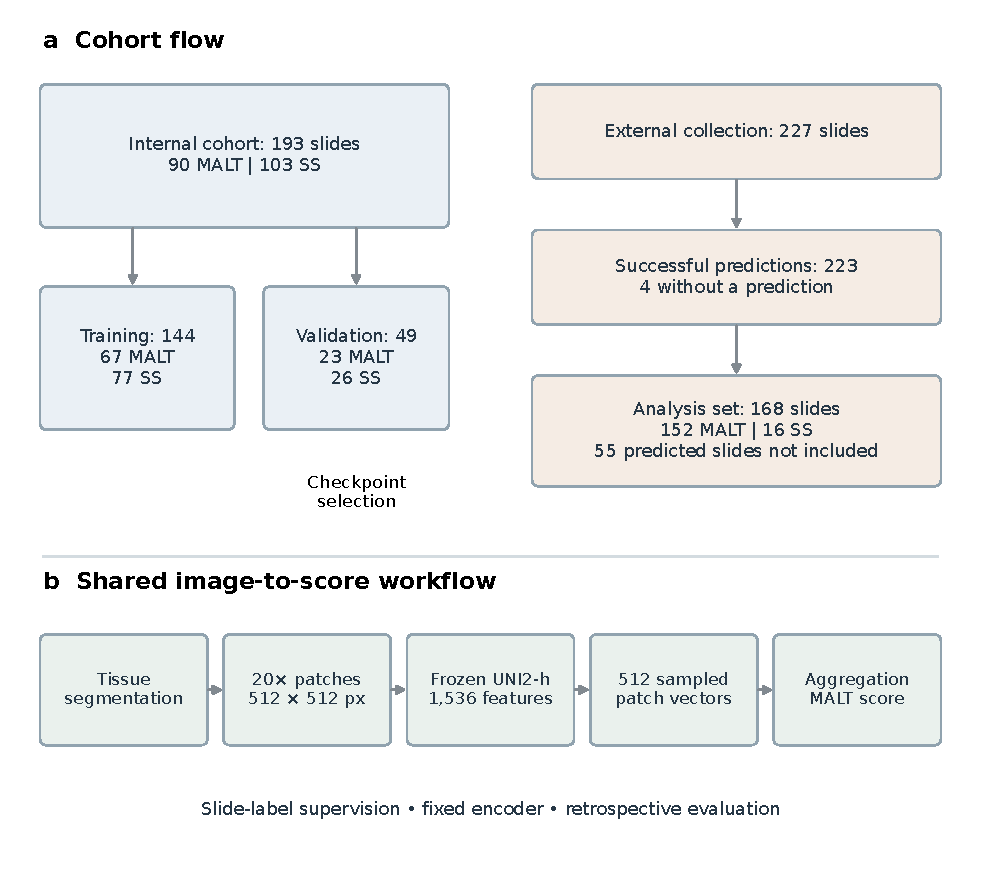
\includegraphics[width=\textwidth]{figures/Figure_1_cohorts.pdf}
\caption{\textbf{Cohort flow and evaluation framework.} All counts are WSIs. The 49-slide validation set was used for checkpoint selection. The external flow distinguishes collection, successful inference and final analysis; clinical exclusion and failure reasons remain completion item H03. The later controlled training and algorithm analyses reused these data and did not create new independent clinical cohorts. The bottom panel summarizes the shared image-to-score workflow; the full Hybrid architecture is detailed in Supplementary Methods.}\label{fig:flow}
\end{figure}


\subsection{The retained model discriminated MALT from SS}
The retained Hybrid checkpoint achieved an internal validation area under the receiver operating characteristic curve (AUROC) of 0.9599 (95\% confidence interval [CI], 0.9046--0.9967). At a score threshold of 0.5, it classified 22/23 MALT and 21/26 SS slides correctly (Fig.~\ref{fig:primary}). External AUROC was 0.8721 (95\% CI, 0.7364--0.9758), with 142/152 MALT and 11/16 SS slides classified correctly. External sensitivity was 93.42\% and specificity was 68.75\%; the specificity interval was wide (44.40\%--85.84\%; Table~\ref{tab:primary}).

ABMIL achieved internal AUROC 0.9498 and external AUROC 0.7903. The paired Hybrid-minus-ABMIL differences were 0.0100 (95\% CI, $-0.0184$ to 0.0452) internally and 0.0818 ($-0.0136$ to 0.2011) externally. External comparisons used identical sampled inputs. Both intervals included zero. These were comparisons of complete implementations with different representation dimensions and training settings, rather than isolated tests of individual Hybrid components. The full historical model comparison, including the separate CONCH v1.5--TITAN pipeline, is provided in Supplementary Table~S1.
\begin{table}[tbp]\centering
\caption{Retained Hybrid performance with conditional 95\% intervals}\label{tab:primary}
\small
\begin{tabular}{>{\raggedright\arraybackslash}p{0.22\textwidth}>{\raggedright\arraybackslash}p{0.34\textwidth}>{\raggedright\arraybackslash}p{0.34\textwidth}}
\toprule
\textbf{Metric} & \textbf{Internal validation} & \textbf{External evaluation} \\
\midrule
AUROC & 0.9599 (0.9046--0.9967) & 0.8721 (0.7364--0.9758) \\
AP & 0.9514 (0.8864--0.9965) & 0.9733 (0.9365--0.9971) \\
Sensitivity & 95.65\% (79.01\%--99.23\%) & 93.42\% (88.31\%--96.39\%) \\
Specificity & 80.77\% (62.12\%--91.49\%) & 68.75\% (44.40\%--85.84\%) \\
Accuracy & 87.76\% (75.76\%--94.27\%) & 91.07\% (85.79\%--94.51\%) \\
PPV & 81.48\% (63.30\%--91.82\%) & 96.60\% (92.29\%--98.54\%) \\
NPV & 95.45\% (78.20\%--99.19\%) & 52.38\% (32.37\%--71.66\%) \\
Balanced accuracy & 88.21\% & 81.09\% \\
\bottomrule\end{tabular}

\par\medskip\footnotesize Threshold metrics use 0.5. AUROC and AP intervals use 2,000 class-stratified WSI bootstrap draws; proportion intervals use Wilson's method. These intervals condition on fitted predictions and do not adjust for selection or patient clustering.
\end{table}

\begin{figure}[tbp]\centering
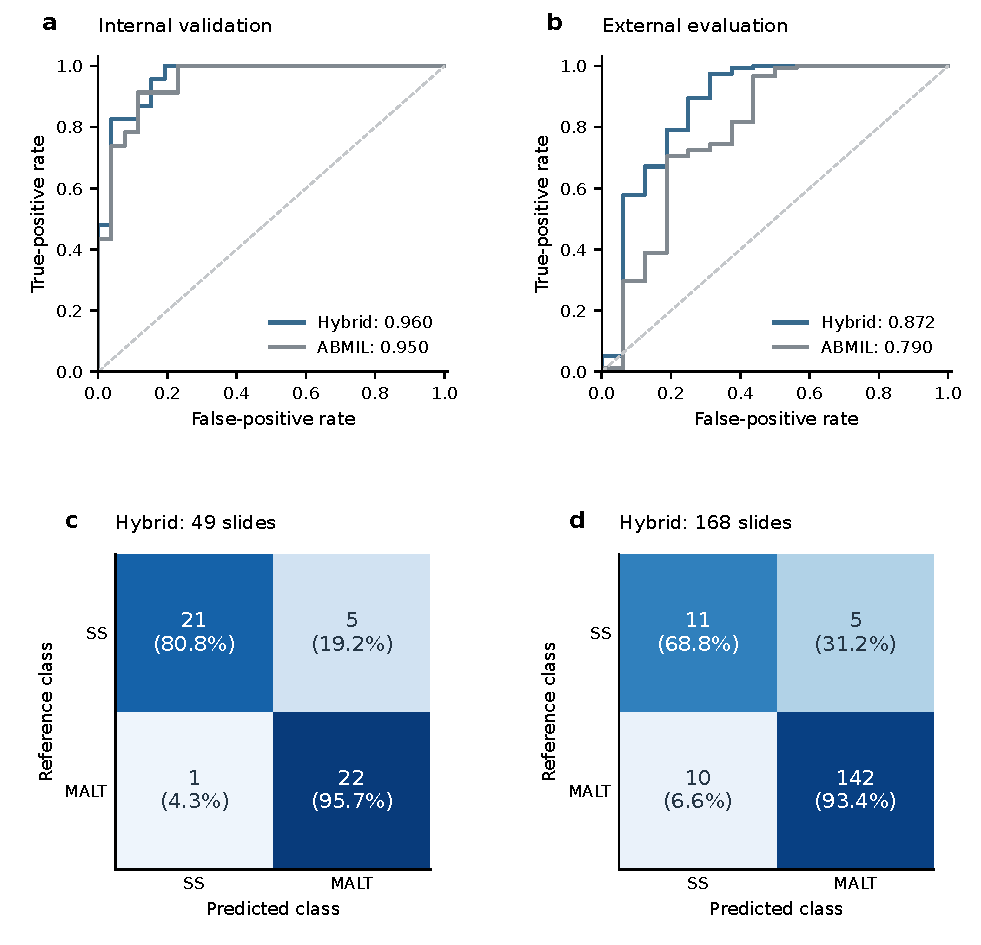
\includegraphics[width=\textwidth]{figures/Figure_2_primary.pdf}
\caption{\textbf{Discrimination and threshold performance of the retained checkpoint.} \textbf{a,b,} ROC curves for Hybrid and ABMIL on internal validation (23 MALT, 26 SS) and external evaluation (152 MALT, 16 SS). External inputs were matched between models. AUROCs describe the retained complete implementations. \textbf{c,d,} Hybrid confusion matrices at threshold 0.5, showing counts and within-reference-class percentages. Validation was used for checkpoint selection. Conditional intervals appear in Table~\ref{tab:primary}; paired AUROC-difference intervals included zero in both cohorts.}\label{fig:primary}
\end{figure}


\subsection{External operating-point performance varied with material composition}
The external MALT fraction was 90.48\%. Overall accuracy of 91.07\% was therefore close to the 90.48\% accuracy of a constant MALT prediction, whereas balanced accuracy was 81.09\%. Average precision (AP) was 0.9733. Of 21 negative model predictions, ten were MALT, giving a negative predictive value (NPV) of 52.38\% (95\% CI, 32.37\%--71.66\%). These quantities describe different aspects of performance in the observed case mix.

Archive categories showed different score distributions (Fig.~\ref{fig:material}). Among source-B MALT slides, 23/33 with H\&E-like tags and 111/111 with immunohistochemistry (IHC)/special-stain tags were positive at threshold 0.5. All eight MALT slides in a separate HE directory were positive. These are archive-derived categories; the stain identity of the SS series was unspecified. In a post hoc descriptive analysis omitting the 111 IHC/special-stain-tagged slides, AUROC was 0.8689, sensitivity was 75.61\% (31/41), and specificity remained 68.75\% (11/16). Thus, the AUROC point estimate was similar while the fixed-threshold MALT detection rate was lower. This subset does not constitute a pathology-confirmed H\&E-only evaluation.

The external Brier score was 0.0919. For context, constant scores equal to the training MALT proportion and the observed external MALT proportion gave descriptive Brier scores of 0.2793 and 0.0862, respectively. The latter uses evaluation labels and is not a deployable comparator. We therefore interpreted the model's Brier score as squared prediction error, not evidence that its scores were calibrated clinical probabilities.
\begin{figure}[tbp]\centering
\fbox{\begin{minipage}[c][35mm][c]{.88\textwidth}\centering
\textbf{Omitted from this public repository copy}\\[6pt]
This figure contains tissue images or individual-slide observations.\\
The complete figure is retained in the local manuscript archive.
\end{minipage}}
\caption{\textbf{External scores in relation to archive categories.} \textbf{a,} Each point is one slide; horizontal segments show medians and the dashed line marks 0.5. Labels give the reference class and sample count. IHC, immunohistochemistry. Categories were derived from archive names and directories, not pathology-confirmed staining. \textbf{b,} Descriptive metrics for all 168 external slides and the 57-slide subset after omitting the IHC/special-stain archive group. The subset contained 41 MALT and all 16 SS slides, whose stain remained unspecified; it is not an H\&E-only validation set. The primary cohort and checkpoint were unchanged.}\label{fig:material}
\end{figure}


\subsection{Controlled comparisons did not establish an aggregation advantage}
Under a common training protocol, matched attention, full fixed scaling and full learned gating had internal AUROC means of 0.9348, 0.9398 and 0.9353 across three seeds. Their external means were 0.7270, 0.7445 and 0.7633, respectively (Supplementary Table~S3). The learned-gate difference from matched attention changed direction across external runs. These results did not establish a consistent benefit from learned gating.

A subsequent screen completed 34 neural-network training runs and two deterministic linear controls. Eight modifications were tested alongside the original Hybrid and matched-attention controls; each configuration initially used three seeds. Attention with input L2 normalization was selected by internal mean AUROC, before the new external inference. Its internal mean of 0.9365 exceeded Hybrid's 0.9353 by 0.0011, below the predefined engineering target of 0.01. Two further seeds were then evaluated for the selected candidate and Hybrid, without changing the selection. Across all five seeds, internal means were 0.9341 and 0.9348, and external means were 0.8061 and 0.8056, respectively (Fig.~\ref{fig:stability}; Table~\ref{tab:controlled}). The candidate used 658,178 parameters compared with Hybrid's 1,521,672, but did not provide a sustained performance gain. All configurations and seeds, including the masking, feature-subspace and consistency experiments, are reported in Supplementary Tables~S4--S5.

Simple linear controls also recovered discriminatory information from the fixed features. Logistic regression on mean features gave external AUROC 0.8335 on the common 512-patch reference inputs; averaging individually L2-normalized features gave 0.8462. Their sensitivities were 45.39\% and 46.05\%, with specificity 93.75\% for both. Full-feature-mean inference yielded AUROCs of 0.8396 and 0.8475 (Supplementary Table~S6). Ranking performance and fixed-threshold sensitivity therefore led to different comparisons.

Probability averaging across all five seeds and five new input bags produced external AUROC 0.8479 for Hybrid and 0.8314 for Attention+L2. The paired candidate-minus-Hybrid difference was $-0.0164$ (95\% CI, $-0.0448$ to 0.0058; Supplementary Table~S7). These ensemble AUROCs are distinct from the mean AUROC across separately trained models.
\begin{table}[tbp]\centering
\caption{Five-seed comparison of Hybrid and the internally selected candidate}\label{tab:controlled}
\small
\begin{tabular}{>{\raggedright\arraybackslash}p{0.19\textwidth}>{\raggedright\arraybackslash}p{0.23\textwidth}>{\raggedright\arraybackslash}p{0.23\textwidth}>{\raggedright\arraybackslash}p{0.12\textwidth}>{\raggedright\arraybackslash}p{0.12\textwidth}}
\toprule
\textbf{Model} & \textbf{Validation AUROC} & \textbf{External AUROC} & \textbf{Ext. sens.} & \textbf{Ext. spec.} \\
\midrule
Hybrid & 0.9348 $\pm$ 0.0134 & 0.8056 $\pm$ 0.1299 & 49.21\% & 82.50\% \\
Attention+L2 & 0.9341 $\pm$ 0.0084 & 0.8061 $\pm$ 0.0916 & 55.66\% & 81.25\% \\
\bottomrule\end{tabular}

\par\medskip\footnotesize AUROCs are means $\pm$ sample SD across seeds 17, 29, 43, 59 and 71; sensitivity and specificity are means of seed-specific rates at 0.5. These are not ensemble metrics. The same 49 validation and 168 external slides were reused. The three-seed selection was fixed before the additional seeds and new external inference.
\end{table}


\subsection{Input sampling affected individual decisions more than aggregate discrimination}
For the retained Hybrid checkpoint, 20 additional patch samples per slide gave internal AUROCs of 0.9498--0.9682 and external AUROCs of 0.8549--0.8943 (Fig.~\ref{fig:stability}). Median per-slide score standard deviations were 0.0120 internally and 0.0150 externally. Nevertheless, seven internal and 18 external slides crossed threshold 0.5 across the 20 draws. Averaging the scores yielded external AUROC 0.8775, with 141 true positives and 12 true negatives: one fewer false positive and one additional false negative than the retained single-bag result (Supplementary Table~S8).

Model-selected regions were linked back to image windows for pathological review (Supplementary Fig.~S4). The maps represent differences in similarity to two latent prototype banks. Their disease-specific morphological meaning has not been established. Performance and visualization runs used different sampled inputs; both scores are retained for the 12 illustrated cases, with no threshold classification changes in those cases (Supplementary Table~S9). Region matching establishes where the displayed patches came from, rather than validating lesion localization.
\begin{figure}[tbp]\centering
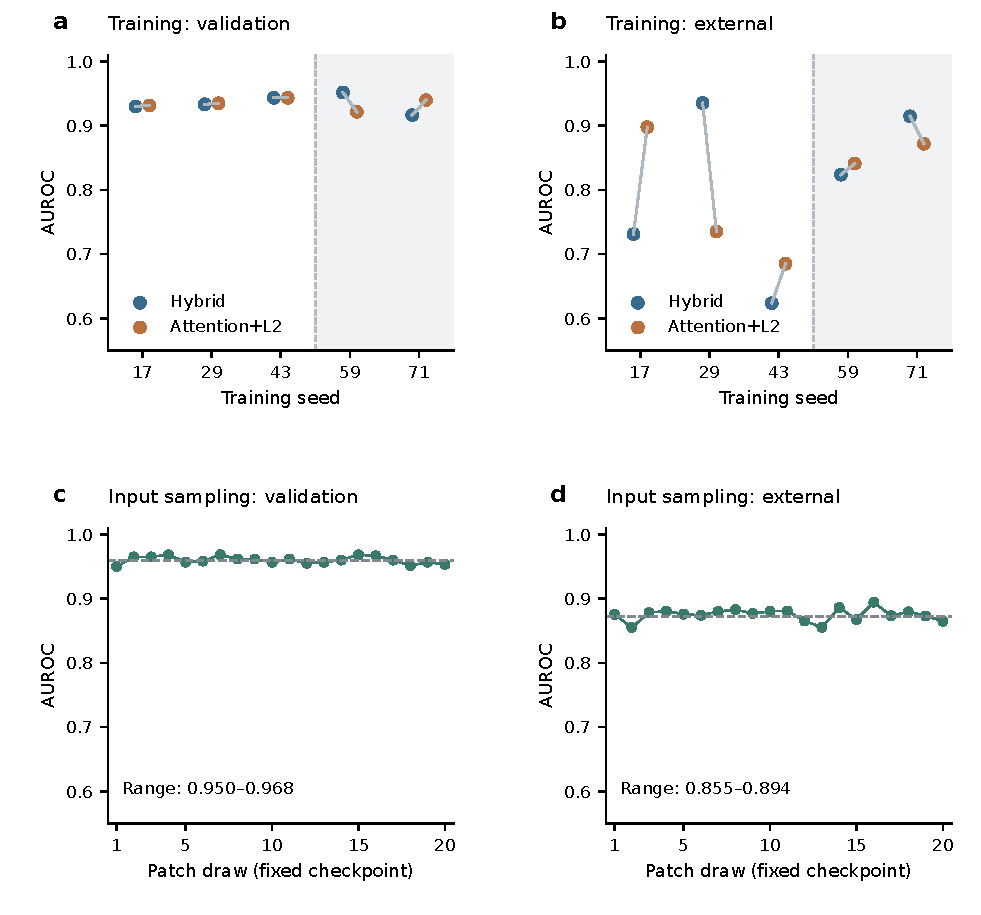
\includegraphics[width=\textwidth]{figures/Figure_4_stability.pdf}
\caption{\textbf{Training and input-sampling variation are different sources of uncertainty.} \textbf{a,b,} AUROC for every training seed of Hybrid and Attention+L2 on internal validation and external evaluation. Gray shading identifies the two additional seeds after candidate selection on the first three internal results. Lines pair model results within each seed; seeds are not independent clinical samples. \textbf{c,d,} AUROC across 20 complete-cohort patch draws for the retained historical Hybrid checkpoint. Dashed lines show its original reference-bag AUROC. These are technical sampling distributions, not confidence intervals; the historical checkpoint differs from the retrained models in a,b. All cohort sizes remain 49 internally and 168 externally.}\label{fig:stability}
\end{figure}

